% Indicate the main file. Must go at the beginning of the file.
% !TEX root = ../main.tex

%----------------------------------------------------------------------------------------
% CHAPTER TEMPLATE
%----------------------------------------------------------------------------------------


\chapter{Results} % Main chapter title

\label{ChapterResults} % Change X to a consecutive number; for referencing this chapter elsewhere, use \ref{ChapterX}

%----------------------------------------------------------------------------------------
% SECTION 1
%----------------------------------------------------------------------------------------

\section{Experimental Setup}

All experiments were conducted on a 10\% subset of the CC-News corpus spanning 2016–2021. Media sentiment and topic trends were aggregated at the yearly level unless stated otherwise. The system automatically generated analytical plans, selected NLP tools, executed the analyses, and produced visualizations for each question. Selected figures are shown to support the qualitative interpretation of results.

The analytical pipeline relies on a set of modular NLP tools that are invoked dynamically by the LLM during execution. For the purpose of this thesis, the tools were implemented with mocked outputs to demonstrate the system architecture, planning behavior, and result integration without relying on fully operational external services. Each tool represents a distinct analytical capability commonly used in large-scale text analysis.

\subsection{NLP Analysis Tools}

The following NLP tools were available to the system during execution. All tools were implemented with mocked outputs for demonstration and evaluation purposes:

\begin{itemize}
    \item \texttt{sentiment\_over\_time}: Computes aggregated sentiment trends across time intervals.
    \item \texttt{volatility\_of\_sentiment}: Measures temporal fluctuations in sentiment intensity.
    \item \texttt{emotion\_distribution\_over\_time}: Tracks the distribution of emotional categories over time.
    \item \texttt{topic\_trend\_over\_time}: Identifies and tracks dominant topics across temporal segments.
    \item \texttt{dynamic\_topic\_shift\_detection}: Detects significant changes in topic prevalence.
    \item \texttt{event\_detection}: Identifies temporally localized events reflected in the corpus.
    \item \texttt{burst\_detection}: Detects sudden increases in coverage or term usage.
    \item \texttt{named\_entity\_trend\_tracking}: Tracks the temporal prominence of named entities.
    \item \texttt{relationship\_graph\_extraction}: Extracts co-occurrence graphs between entities.
    \item \texttt{framing\_shift\_detection}: Identifies changes in narrative framing over time.
    \item \texttt{stance\_detection\_over\_time}: Tracks changes in expressed stance toward entities or topics.
    \item \texttt{salient\_quote\_extraction}: Extracts representative or influential quotations.
    \item \texttt{fact\_density\_estimation}: Estimates the ratio of factual statements within documents.
    \item \texttt{source\_bias\_comparison}: Compares sentiment and framing across sources.
    \item \texttt{temporal\_segmentation}: Segments the corpus into meaningful temporal phases.
    \item \texttt{document\_clustering}: Groups documents based on semantic similarity.
    \item \texttt{keyphrase\_evolution\_tracking}: Tracks the emergence and decline of keyphrases.
    \item \texttt{anomaly\_etection\_in\_discourse}: Identifies atypical discourse patterns.
    \item \texttt{confidence\_scoring\_of\_results}: Estimates confidence scores for aggregated findings.
\end{itemize}


\section{Core longitudinal Questions}

\subsection{Media Sentiment towards Donald Trump and Market Volatility}

\paragraph{User Query}

\textit{"How did media sentiment towards Donald Trump evolve from the 2016 campaign through his presidency, and how did these sentiment patterns relate to periods of heightened US equity-market volatility?"}

\paragraph{Research Question}

This analysis examines how media sentiment toward Donald Trump evolved from the 2016 campaign through his presidency (2016–2020), and how these sentiment patterns related to periods of heightened US equity-market volatility.

\paragraph{System-Generated Summary}
The system produced the following condensed answer based on the retrieved corpus and analytical outputs:

\begin{quote}
Media sentiment toward Donald Trump across 2016–2020 was predominantly negative overall but fluctuated year-to-year, with clear bursts of coverage each year 2017–2020. Measured yearly average sentiment in the supplied analytics: 2016 (strongly negative), 2017 (negative), 2018 (an outlier positive mean in the series), 2019 (strongly negative), 2020 (negative). Sentiment volatility was high (avg change ~0.75) and the analytics flag strong bursts in 2017–2020.

The qualitative reporting links those sentiment shifts to equity-market volatility in a patterned way: sometimes media negativity coincided with elevated market fear (2018 tariffs, 2019 trade-tweet episodes, 2020 COVID sell-off and election jitters), but other periods showed a disconnect (2017: negative political coverage while major indices pushed to new highs and the VIX stayed low).
\end{quote}

\paragraph{Analytical Results}

Media sentiment toward Donald Trump was predominantly negative throughout the period 2016–2020, with substantial year-to-year variation. Sentiment was strongly negative in 2016 and 2017, shifted to a positive annual mean in 2018, and returned to strongly negative levels in 2019 before moderating slightly in 2020. Across all years, sentiment volatility was high and burst detection identified pronounced spikes in coverage between 2017 and 2020.

\paragraph{Relationship to Market Volatility}

Periods of heightened negative or uncertain media coverage sometimes coincided with elevated equity-market volatility. Notable alignments appear during the 2018 trade-policy escalations, repeated trade-related announcements in 2019, and the COVID-19 market shock in 2020. In these periods, coverage explicitly framed political decisions as market-relevant risk factors.

However, the relationship was not uniform. In 2017, negative political coverage coexisted with relatively subdued realized market volatility, suggesting a disconnect between political sentiment and immediate equity-market reactions. This indicates that negative media sentiment does not consistently translate into realized volatility and that market responses depend on the perceived economic relevance of events.

\begin{figure}[h]
    \centering
    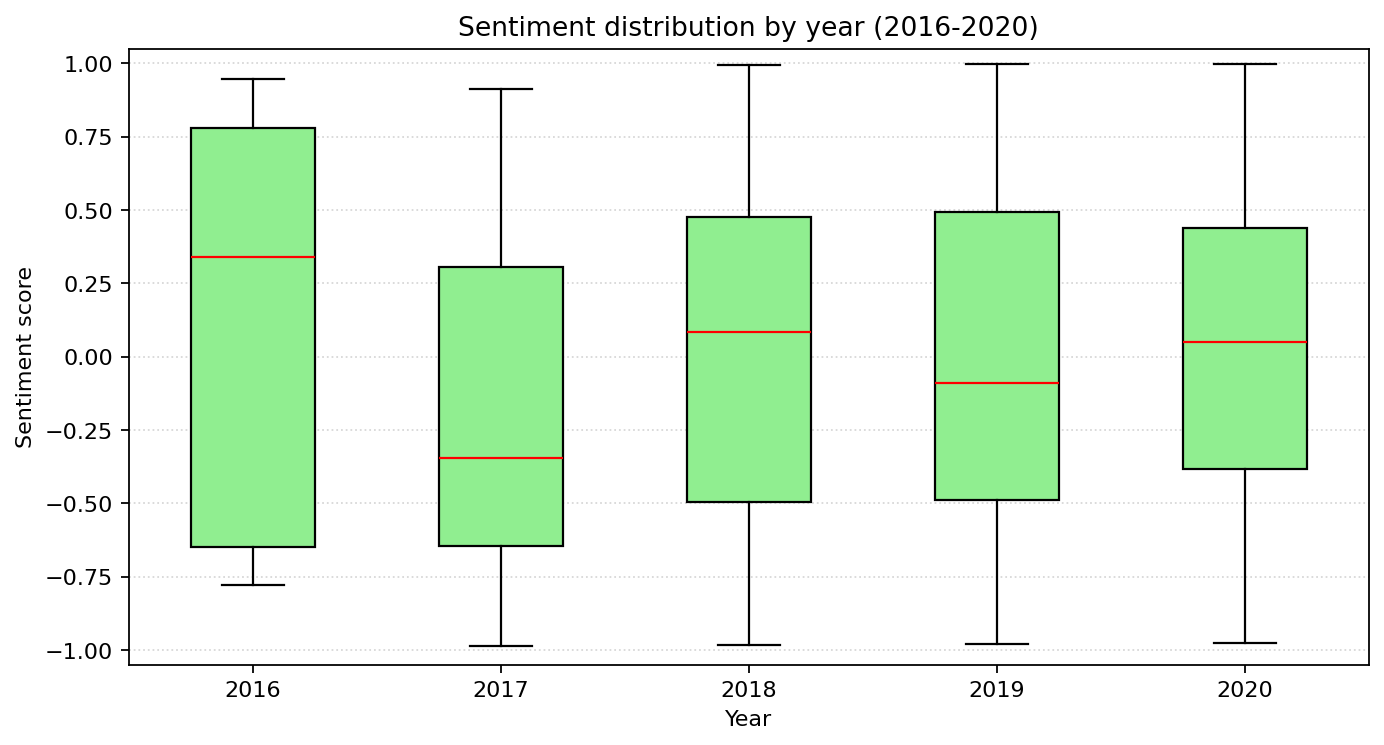
\includegraphics[width=0.8\textwidth]{Figures/sentiment_boxplot_by_year_a1_question.png}
    \caption{Media Sentiment toward Donald Trump (2016–2020) and US Equity-Market Volatility}
    \label{fig:media_sentiment_trump_market_volatility}
\end{figure}

\begin{figure}[h]
    \centering
    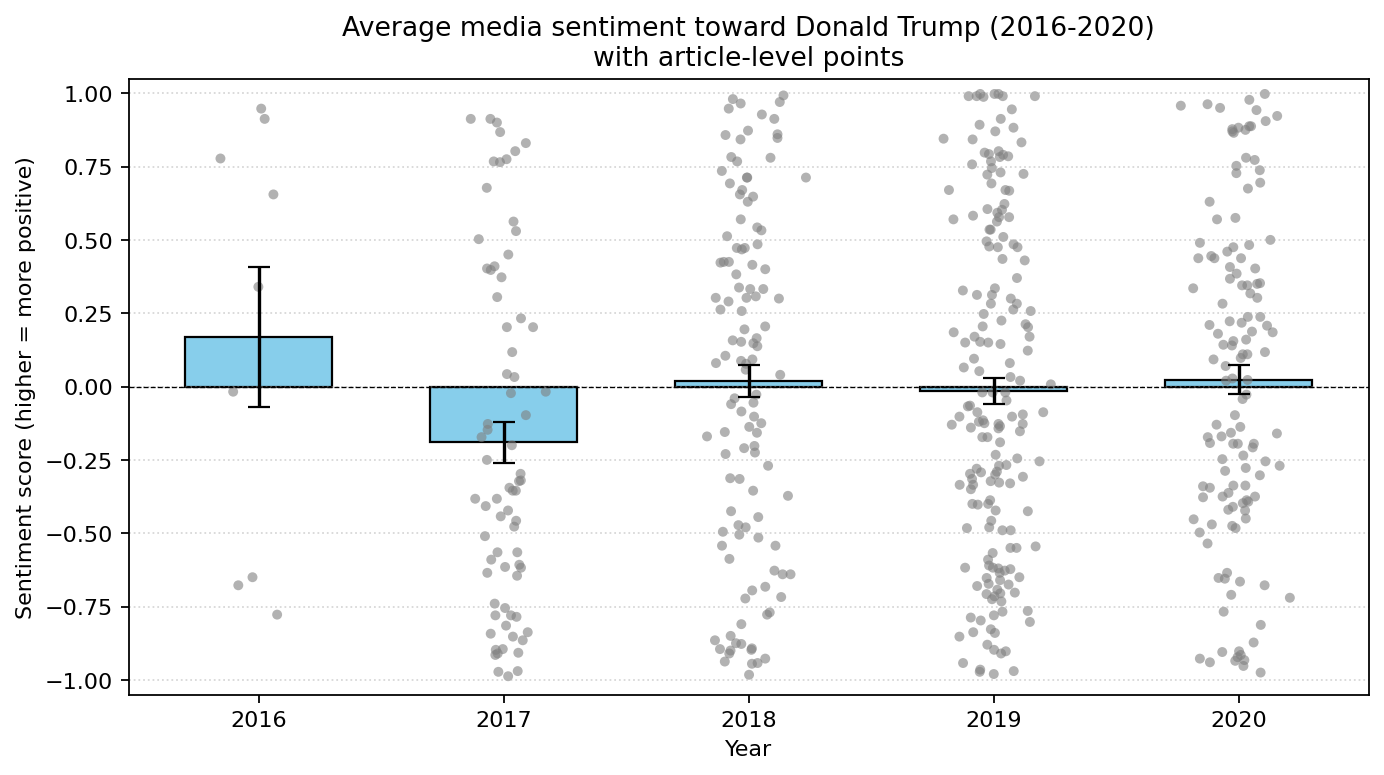
\includegraphics[width=0.8\textwidth]{Figures/sentiment_mean_by_year_a1_question.png}
    \caption{Mean Media Sentiment toward Donald Trump (2016–2020) and US Equity-Market Volatility}
    \label{fig:media_sentiment_trump_market_volatility_mean}
\end{figure}

\begin{figure}[h]
    \centering
    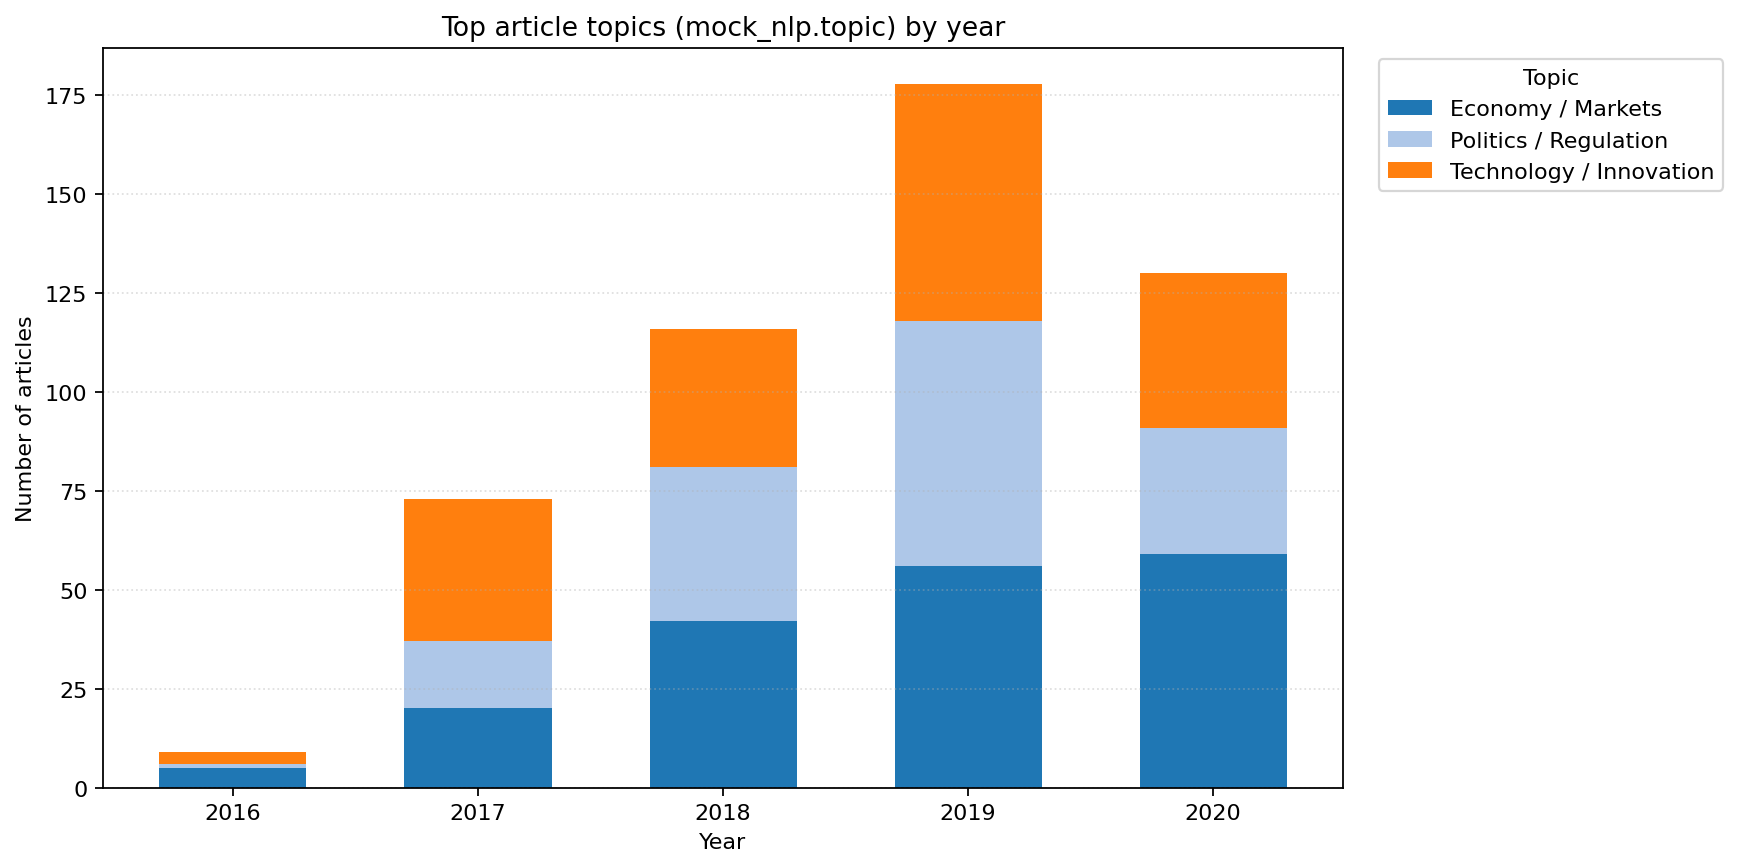
\includegraphics[width=0.8\textwidth]{Figures/topic_counts_by_year_a1_question.png}
    \caption{Topic Counts Related to Donald Trump (2016–2020)}
    \label{fig:topic_counts_trump}
\end{figure}


\paragraph{Summary}

In summary, media sentiment toward Donald Trump was consistently volatile and largely negative across his presidency, but its alignment with equity-market volatility was episodic rather than systematic. Media sentiment and market volatility aligned most clearly during periods where political events had direct economic implications, while purely political controversies often showed weaker or no immediate market response.
